\documentclass{../exercisesheet}

\title{Datenkommunikation und Informationssysteme, Übung 6}
\author{
    Domenic Quirl \\ 354437
    \and
    Julian Schakib \\ 353889
    \and 
    Daniel Schleiz \\ 356092
}

\renewcommand{\Exercise}{Aufgabe}
\date{Übungsgruppe 14}

\usepackage{float}
%\usepackage{siunitx}
\usepackage{color}
\usepackage{multirow}
\usepackage{float}

\begin{document}
\maketitle
\pointtable


\begin{exercise}{4}
\begin{subexercise}

\end{subexercise}
\begin{subexercise}

\end{subexercise}
\begin{subexercise}

\end{subexercise}
\end{exercise}


\begin{exercise}{6}
\begin{subexercise}

\end{subexercise}
\begin{subexercise}

\end{subexercise}
\begin{subexercise}

\end{subexercise}
\begin{subexercise}

\end{subexercise}
\end{exercise}


\begin{exercise}{5}
\begin{subexercise}
\begin{figure}[H]
  \centering
  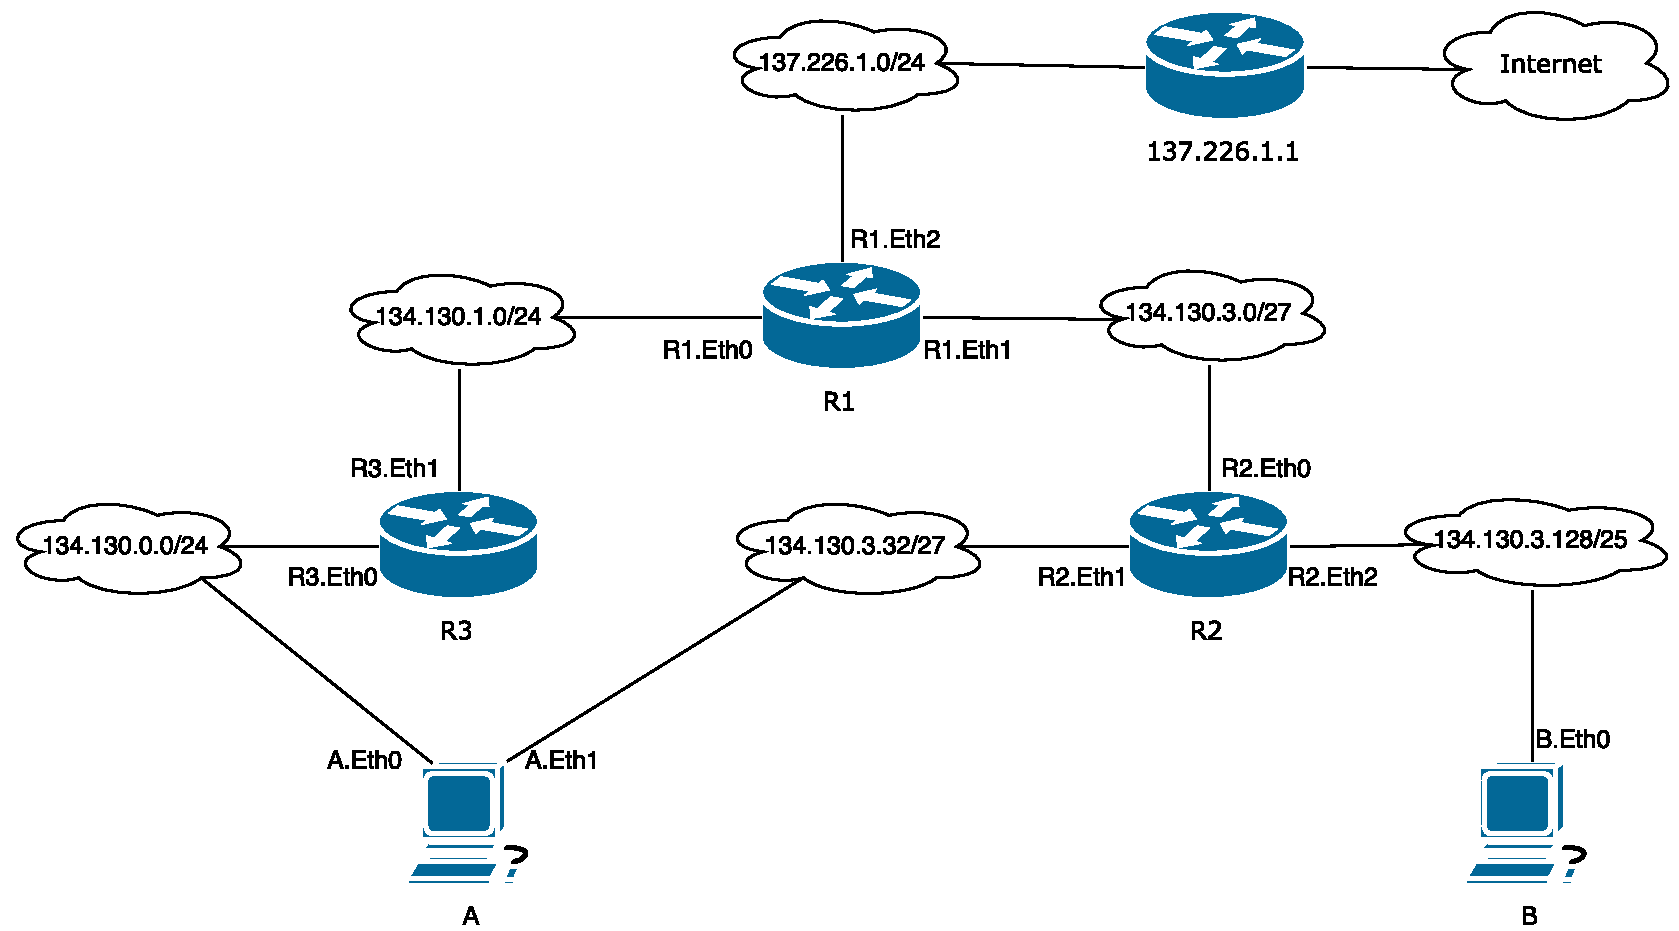
\includegraphics[width=\textwidth]{a3_network.pdf}
\end{figure}
\end{subexercise}
\begin{subexercise}
Der längste Match der IP-Adresse von B in der Tabelle von A besteht bei \texttt{0.0.0.0/0}, somit sendet A durch ETH0.\\ \ \\
\begin{tt}
Request A.ETH0 134.130.0.152
\end{tt}
\end{subexercise}
\end{exercise}


\end{document}

